% Options for packages loaded elsewhere
% Options for packages loaded elsewhere
\PassOptionsToPackage{unicode}{hyperref}
\PassOptionsToPackage{hyphens}{url}
\PassOptionsToPackage{dvipsnames,svgnames,x11names}{xcolor}
%
\documentclass[
  letterpaper,
]{article}
\usepackage{xcolor}
\usepackage{amsmath,amssymb}
\setcounter{secnumdepth}{5}
\usepackage{iftex}
\ifPDFTeX
  \usepackage[T1]{fontenc}
  \usepackage[utf8]{inputenc}
  \usepackage{textcomp} % provide euro and other symbols
\else % if luatex or xetex
  \usepackage{unicode-math} % this also loads fontspec
  \defaultfontfeatures{Scale=MatchLowercase}
  \defaultfontfeatures[\rmfamily]{Ligatures=TeX,Scale=1}
\fi
\usepackage{lmodern}
\ifPDFTeX\else
  % xetex/luatex font selection
  \setmainfont[]{Latin Modern Sans}
  \setsansfont[]{Latin Modern Sans}
\fi
% Use upquote if available, for straight quotes in verbatim environments
\IfFileExists{upquote.sty}{\usepackage{upquote}}{}
\IfFileExists{microtype.sty}{% use microtype if available
  \usepackage[]{microtype}
  \UseMicrotypeSet[protrusion]{basicmath} % disable protrusion for tt fonts
}{}
\makeatletter
\@ifundefined{KOMAClassName}{% if non-KOMA class
  \IfFileExists{parskip.sty}{%
    \usepackage{parskip}
  }{% else
    \setlength{\parindent}{0pt}
    \setlength{\parskip}{6pt plus 2pt minus 1pt}}
}{% if KOMA class
  \KOMAoptions{parskip=half}}
\makeatother
% Make \paragraph and \subparagraph free-standing
\makeatletter
\ifx\paragraph\undefined\else
  \let\oldparagraph\paragraph
  \renewcommand{\paragraph}{
    \@ifstar
      \xxxParagraphStar
      \xxxParagraphNoStar
  }
  \newcommand{\xxxParagraphStar}[1]{\oldparagraph*{#1}\mbox{}}
  \newcommand{\xxxParagraphNoStar}[1]{\oldparagraph{#1}\mbox{}}
\fi
\ifx\subparagraph\undefined\else
  \let\oldsubparagraph\subparagraph
  \renewcommand{\subparagraph}{
    \@ifstar
      \xxxSubParagraphStar
      \xxxSubParagraphNoStar
  }
  \newcommand{\xxxSubParagraphStar}[1]{\oldsubparagraph*{#1}\mbox{}}
  \newcommand{\xxxSubParagraphNoStar}[1]{\oldsubparagraph{#1}\mbox{}}
\fi
\makeatother


\usepackage{longtable,booktabs,array}
\newcounter{none} % for unnumbered tables
\usepackage{calc} % for calculating minipage widths
% Correct order of tables after \paragraph or \subparagraph
\usepackage{etoolbox}
\makeatletter
\patchcmd\longtable{\par}{\if@noskipsec\mbox{}\fi\par}{}{}
\makeatother
% Allow footnotes in longtable head/foot
\IfFileExists{footnotehyper.sty}{\usepackage{footnotehyper}}{\usepackage{footnote}}
\makesavenoteenv{longtable}
\usepackage{graphicx}
\makeatletter
\newsavebox\pandoc@box
\newcommand*\pandocbounded[1]{% scales image to fit in text height/width
  \sbox\pandoc@box{#1}%
  \Gscale@div\@tempa{\textheight}{\dimexpr\ht\pandoc@box+\dp\pandoc@box\relax}%
  \Gscale@div\@tempb{\linewidth}{\wd\pandoc@box}%
  \ifdim\@tempb\p@<\@tempa\p@\let\@tempa\@tempb\fi% select the smaller of both
  \ifdim\@tempa\p@<\p@\scalebox{\@tempa}{\usebox\pandoc@box}%
  \else\usebox{\pandoc@box}%
  \fi%
}
% Set default figure placement to htbp
\def\fps@figure{htbp}
\makeatother


% definitions for citeproc citations
\NewDocumentCommand\citeproctext{}{}
\NewDocumentCommand\citeproc{mm}{%
  \begingroup\def\citeproctext{#2}\cite{#1}\endgroup}
\makeatletter
 % allow citations to break across lines
 \let\@cite@ofmt\@firstofone
 % avoid brackets around text for \cite:
 \def\@biblabel#1{}
 \def\@cite#1#2{{#1\if@tempswa , #2\fi}}
\makeatother
\newlength{\cslhangindent}
\setlength{\cslhangindent}{1.5em}
\newlength{\csllabelwidth}
\setlength{\csllabelwidth}{3em}
\newenvironment{CSLReferences}[2] % #1 hanging-indent, #2 entry-spacing
 {\begin{list}{}{%
  \setlength{\itemindent}{0pt}
  \setlength{\leftmargin}{0pt}
  \setlength{\parsep}{0pt}
  % turn on hanging indent if param 1 is 1
  \ifodd #1
   \setlength{\leftmargin}{\cslhangindent}
   \setlength{\itemindent}{-1\cslhangindent}
  \fi
  % set entry spacing
  \setlength{\itemsep}{#2\baselineskip}}}
 {\end{list}}
\usepackage{calc}
\newcommand{\CSLBlock}[1]{\hfill\break\parbox[t]{\linewidth}{\strut\ignorespaces#1\strut}}
\newcommand{\CSLLeftMargin}[1]{\parbox[t]{\csllabelwidth}{\strut#1\strut}}
\newcommand{\CSLRightInline}[1]{\parbox[t]{\linewidth - \csllabelwidth}{\strut#1\strut}}
\newcommand{\CSLIndent}[1]{\hspace{\cslhangindent}#1}



\setlength{\emergencystretch}{3em} % prevent overfull lines

\providecommand{\tightlist}{%
  \setlength{\itemsep}{0pt}\setlength{\parskip}{0pt}}



 


\usepackage{hyphenat}
\usepackage{graphicx}
% and their extensions so you won't have to specify these with
 % every instance of \includegraphics
\usepackage{pdfcomment}
\DeclareGraphicsExtensions{.pdf,.jpeg,.png}
\usepackage{wallpaper} % for the background image on title page
\usepackage{geometry}

\usepackage{lastpage}
% set font
% \usepackage{fontspec}
% \setsansfont{Latin Modern Sans}
% \renewcommand{\setmainfont}[2][]{\fontspec[#1]{Latin Modern Sans}}
% \renewcommand{\rmdefault}{lmss}

% Acronyms
\usepackage[acronym]{glossaries}
\glsdisablehyper
\makenoidxglossaries
\loadglsentries{report_glossary.tex}

% \usepackage{lmodern}
\usepackage[T1]{fontenc}

\newfontfamily\sectionfont[Color=Black]{Latin Modern Sans}
\newfontfamily\subsectionfont[Color=Black]{Latin Modern Sans}
\newfontfamily\subsubsectionfont[Color=Black]{Latin Modern Sans}
% \addtokomafont{section}{\sectionfont}
% \addtokomafont{subsection}{\subsectionfont}
% \addtokomafont{subsubsection}{\subsubsectionfont}
\usepackage[headsepline=0.005pt:,footsepline=0.005pt:,plainfootsepline,automark]{scrlayer-scrpage}
\clearpairofpagestyles
\ohead[]{\headmark} \cofoot[\pagemark]{\pagemark}
\lohead{Petrale sole assessment 2023}
\ModifyLayer[addvoffset=-.6ex]{scrheadings.foot.above.line}
\ModifyLayer[addvoffset=-.6ex]{plain.scrheadings.foot.above.line}
\setkomafont{pageheadfoot}{\small}

% add soul package to remove latex error
\usepackage{soul}

\usepackage{float}
\floatplacement{table}{H}

\usepackage{booktabs}
\usepackage{caption}
\usepackage{longtable}
\usepackage{colortbl}
\usepackage{array}
\usepackage{anyfontsize}
\usepackage{multirow}
\makeatletter
\@ifpackageloaded{caption}{}{\usepackage{caption}}
\AtBeginDocument{%
\ifdefined\contentsname
  \renewcommand*\contentsname{Table of contents}
\else
  \newcommand\contentsname{Table of contents}
\fi
\ifdefined\listfigurename
  \renewcommand*\listfigurename{List of Figures}
\else
  \newcommand\listfigurename{List of Figures}
\fi
\ifdefined\listtablename
  \renewcommand*\listtablename{List of Tables}
\else
  \newcommand\listtablename{List of Tables}
\fi
\ifdefined\figurename
  \renewcommand*\figurename{Figure}
\else
  \newcommand\figurename{Figure}
\fi
\ifdefined\tablename
  \renewcommand*\tablename{Table}
\else
  \newcommand\tablename{Table}
\fi
}
\@ifpackageloaded{float}{}{\usepackage{float}}
\floatstyle{ruled}
\@ifundefined{c@chapter}{\newfloat{codelisting}{h}{lop}}{\newfloat{codelisting}{h}{lop}[chapter]}
\floatname{codelisting}{Listing}
\newcommand*\listoflistings{\listof{codelisting}{List of Listings}}
\makeatother
\makeatletter
\usepackage{pdflscape}
\makeatother
\makeatletter
\makeatother
\makeatletter
\@ifpackageloaded{caption}{}{\usepackage{caption}}
\@ifpackageloaded{subcaption}{}{\usepackage{subcaption}}
\makeatother
\usepackage{bookmark}
\IfFileExists{xurl.sty}{\usepackage{xurl}}{} % add URL line breaks if available
\urlstyle{same}
\hypersetup{
  pdftitle={Status of Petrale sole stock off the U.S. West Coast in 2023},
  pdfauthor={Ian G. Taylor; Vladlena Gertseva; Nick Tolimieri},
  colorlinks=true,
  linkcolor={blue},
  filecolor={Maroon},
  citecolor={Blue},
  urlcolor={Blue},
  pdfcreator={LaTeX via pandoc}}


\title{Status of Petrale sole stock off the U.S. West Coast in 2023}
\author{Ian G. Taylor \and Vladlena Gertseva \and Nick Tolimieri}
\date{2026-07-20}
\begin{document}
  \begin{titlepage}
  % This is a combination of Pandoc templating and LaTeX
  % Pandoc templating https://pandoc.org/MANUAL.html#templates
  % See the README for help

  \newgeometry{top=2in,bottom=1in,right=1in,left=1in}
  \begin{minipage}[b][\textheight][s]{\textwidth}
  % Ross would've subbed lines 6, 8 with these lines:
  %\newgeometry{top=2in,bottom=1in,right=1in,left=1in}%
  %\noindent  %\tracingall
  %\begin{minipage}[b][\textheight][s]{.975\textwidth}%% RRM: avoid Overfull box


  \raggedright

  % \includegraphics[width=2cm]{NOAA_Transparent_Logo.png}

  % background image


  % Title and subtitle
  {\huge\bfseries\nohyphens{Status of Petrale sole stock off the U.S.
  West Coast in 2023}}\\[1\baselineskip]
  % Ross would change the end of the above line to the following because \par must come before the group closes and line-depth reverts.
  % }\par}%\\[1\baselineskip]



  \vspace{2\baselineskip}
  % Ross would change this to 2\baselineskip

  %%%%%% Cover image
  \pandocbounded{\includegraphics[width=6in, alt=An illustration of Petrale sole.]{support\_files/Petrale\_sole.png}}
  % cover page customization need to be inserted here
  %\pdftooltip{\includegraphics{support\_files/Petrale\_sole.png}}{Alt text}

  \vspace{1\baselineskip}

  % Authors
  % This hairy bit of code is just to get "and" between the last 2
  % authors. See below if you don't need that
   {\large{Ian G. Taylor}}{\textsuperscript{1}}%
  %
  ,
   {\large{Vladlena Gertseva}}{\textsuperscript{1}}%
  %
  %
  { and \large{Nick Tolimieri}}%
  {\textsuperscript{1}}%
  %


  % This is how to do it if you don't need the "and"

  %%%%%% Affiliations
  \vspace{2\baselineskip}

  \hangindent=1em
  \hangafter=1
  % Ross would change the above line to:
  % \hangafter=1\relax
  %
  {1}.~{NOAA Fisheries Northwest Fisheries Science Center}%
  %
  %
    , %
    2725 Montlake Boulevard East, Seattle, WA, 98112-2097%
  %


  %%%%%% Correspondence
  \vspace{1\baselineskip}


  %use \vfill instead to get the space to fill flexibly
  %\vspace{0.25\textheight} % Whitespace between the title block and the publisher

  \vfill


  % Whitespace between the title block and the tagline
  \vspace{1\baselineskip}

  %%%%%% Tagline at bottom
  % Ross says the tagline below could also be centered
  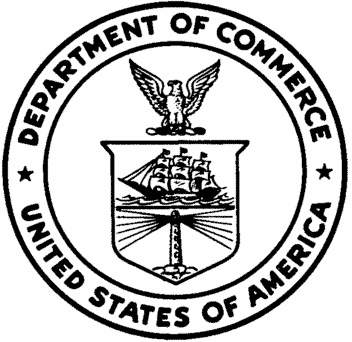
\includegraphics[width=2cm, artifact]{support_files/us_doc_logo.png}\newline % empty curly brackets without alt text is suitable for this logo because it's purely decorative/an "artifact"
  U.S. Department of Commerce\newline
  National Oceanic and Atmospheric Administration\newline
  National Marine Fisheries Service\newline
  Northwest Fisheries Science Center\newline

  \end{minipage}
  \restoregeometry
  \end{titlepage}

\newgeometry{top=1in,bottom=1in,right=1in,left=1in}

\pdfbookmark[1]{Table of Contents}{toc}
\renewcommand*\contentsname{Table of contents}
{
\setcounter{tocdepth}{3}
\tableofcontents
}
\listoffigures
\listoftables

\printnoidxglossaries

\newpage{}

\subsection*{Disclaimer}\label{disclaimer}

These materials do not constitute a formal publication and are for
information only. They are in a pre-review, pre-decisional state and
should not be formally cited or reproduced. They are to be considered
provisional and do not represent any determination or policy of NOAA or
the Department of Commerce.

\newpage{}

Please cite this publication as:

Taylor, I. G., Gertseva, V., and Tolimieri, N. 2023. Status of Petrale
sole stock off the U.S. West Coast in 2023. Prepared by {[}COMMITTEE{]}.
\pageref*{LastPage}{} pp.

\newpage{}

\section{Data}\label{sec-data}

\subsection{Life History}\label{life-history}

\subsection{Catch}\label{catch}

\subsection{Indices and
Standardization}\label{indices-and-standardization}

\subsection{Composition Data}\label{composition-data}

\subsection{Absolute Abundance}\label{absolute-abundance}

\subsection{Environmental/Ecosystem Indicator
Data}\label{environmentalecosystem-indicator-data}

\newpage{}

\section{Assessment}\label{sec-assmt-config}

\subsection{Current Modeling Approach}\label{current-modeling-approach}

\subsection{Configuration of the Base
Model}\label{configuration-of-the-base-model}

\subsection{Bridging}\label{bridging}

\newpage{}

\subsection{Modeling Results}\label{sec-assmt-results}

\subsubsection{Parameter Estimates}\label{parameter-estimates}

\subsubsection{Time Series}\label{time-series}

\subsubsection{Model Fits}\label{model-fits}

\subsubsection{Model Diagnostics}\label{model-diagnostics}

\newpage{}

\subsection{Sensitivity Analyses}\label{sec-assmt-sens}

\newpage{}

\subsection{Management Benchmarks}\label{sec-assmt-bench}

\newpage{}

\subsection{Projections}\label{sec-assmt-proj}

\newpage{}

\subsection{Harvest Control Rules}\label{harvest-control-rules}

{[}Insert text here{]}

\newpage{}

\section{Discussion}\label{sec-discussion}

\newpage{}

\section{Acknowledgements}\label{sec-acknowledgements}

This document was produced using the R package asar (Schiano et al.
2026), which is free to use and publicly available on
\href{https://github.com/nmfs-ost/asar}{GitHub}.

\newpage{}

\section{References}\label{sec-refs}

\protect\phantomsection\label{refs}
\begin{CSLReferences}{1}{0}
\bibitem[\citeproctext]{ref-asar_2026}
Schiano, S., Breitbart, S., and Saul, S. 2026. Asar: Build NOAA stock
assessment report. Available from
\url{https://github.com/nmfs-ost/asar}.

\end{CSLReferences}

\newpage{}

\section{Tables}\label{sec-tables}

\begin{landscape}

\begin{table}[t]

\caption{\label{tbl-index}Calculated index of abundance and
corresponding CVs for the fleets and surveys identified in the column
headers.}

\centering{

\fontsize{12.0pt}{14.0pt}\selectfont
\begin{tabular*}{1\linewidth}{@{\extracolsep{\fill}}>{\centering\arraybackslash}p{\dimexpr 0.20\linewidth -2\tabcolsep-1.5\arrayrulewidth}>{\centering\arraybackslash}p{\dimexpr 0.20\linewidth -2\tabcolsep-1.5\arrayrulewidth}>{\centering\arraybackslash}p{\dimexpr 0.20\linewidth -2\tabcolsep-1.5\arrayrulewidth}>{\centering\arraybackslash}p{\dimexpr 0.20\linewidth -2\tabcolsep-1.5\arrayrulewidth}>{\centering\arraybackslash}p{\dimexpr 0.20\linewidth -2\tabcolsep-1.5\arrayrulewidth}}
\toprule
{\bfseries Year} & {\bfseries Index Observed Triennial (se)} & {\bfseries Index Predicted Triennial (se)} & {\bfseries Index Observed Wcgbts (se)} & {\bfseries Index Predicted Wcgbts (se)} \\ 
\midrule\addlinespace[2.5pt]
1980 & 1,835.00 (0.38) & 3,322.83 (0.38) & - & - \\ 
1983 & 1,968.45 (0.34) & 2,438.46 (0.34) & - & - \\ 
1986 & 1,819.10 (0.34) & 2,211.88 (0.34) & - & - \\ 
1989 & 2,590.42 (0.34) & 2,177.91 (0.34) & - & - \\ 
1992 & 1,860.61 (0.34) & 1,933.47 (0.34) & - & - \\ 
1995 & 2,071.20 (0.35) & 2,516.70 (0.35) & - & - \\ 
1998 & 3,071.65 (0.33) & 2,784.97 (0.33) & - & - \\ 
2001 & 3,411.62 (0.34) & 3,298.33 (0.34) & - & - \\ 
2004 & 8,975.17 (0.34) & 4,051.63 (0.34) & 22,772.20 (0.09) & 20,790.60 (0.09) \\ 
2003 & - & - & 18,526.50 (0.09) & 19,373.70 (0.09) \\ 
2005 & - & - & 23,426.80 (0.08) & 20,698.20 (0.08) \\ 
2006 & - & - & 21,032.50 (0.08) & 19,167.60 (0.08) \\ 
2007 & - & - & 18,081.30 (0.08) & 17,844.10 (0.08) \\ 
2008 & - & - & 16,272.40 (0.08) & 17,074.90 (0.08) \\ 
2009 & - & - & 16,343.10 (0.08) & 17,896.00 (0.08) \\ 
2010 & - & - & 23,898.40 (0.07) & 22,500.50 (0.07) \\ 
2011 & - & - & 31,344.10 (0.07) & 30,760.20 (0.07) \\ 
2012 & - & - & 36,896.00 (0.07) & 40,647.60 (0.07) \\ 
2013 & - & - & 55,341.80 (0.09) & 49,036.70 (0.09) \\ 
2014 & - & - & 57,060.90 (0.07) & 54,277.90 (0.07) \\ 
2015 & - & - & 51,353.50 (0.07) & 56,914.90 (0.07) \\ 
2016 & - & - & 59,009.80 (0.07) & 57,499.30 (0.07) \\ 
2017 & - & - & 60,348.00 (0.07) & 56,575.70 (0.07) \\ 
2018 & - & - & 42,010.00 (0.08) & 54,735.80 (0.08) \\ 
2019 & - & - & 43,739.20 (0.1) & 52,972.80 (0.1) \\ 
2021 & - & - & 50,087.90 (0.07) & 49,724.90 (0.07) \\ 
2022 & - & - & 51,429.80 (0.08) & 45,694.10 (0.08) \\ 
\bottomrule
\end{tabular*}

}

\end{table}%

\end{landscape}

\newpage{}

\begin{landscape}

\begin{table}[t]

\caption{\label{tbl-landings1}Landed catch by fleet and year in mt. (1
of 6)}

\centering{

\fontsize{12.0pt}{14.0pt}\selectfont
\begin{tabular*}{1\linewidth}{@{\extracolsep{\fill}}>{\centering\arraybackslash}p{\dimexpr 0.20\linewidth -2\tabcolsep-1.5\arrayrulewidth}>{\centering\arraybackslash}p{\dimexpr 0.20\linewidth -2\tabcolsep-1.5\arrayrulewidth}>{\centering\arraybackslash}p{\dimexpr 0.20\linewidth -2\tabcolsep-1.5\arrayrulewidth}>{\centering\arraybackslash}p{\dimexpr 0.20\linewidth -2\tabcolsep-1.5\arrayrulewidth}>{\centering\arraybackslash}p{\dimexpr 0.20\linewidth -2\tabcolsep-1.5\arrayrulewidth}}
\toprule
{\bfseries Year} & {\bfseries Landings Observed Weight North  (mt) (se)} & {\bfseries Landings Predicted Weight North  (mt) (se)} & {\bfseries Landings Observed Weight South  (mt) (se)} & {\bfseries Landings Predicted Weight South  (mt) (se)} \\ 
\midrule\addlinespace[2.5pt]
1876 & 0.00 (0.01) & 0.00 (0.01) & 1.00 (0.01) & 1.00 (0.01) \\ 
1877 & 0.00 (0.01) & 0.00 (0.01) & 1.00 (0.01) & 1.00 (0.01) \\ 
1878 & 0.00 (0.01) & 0.00 (0.01) & 1.00 (0.01) & 1.00 (0.01) \\ 
1879 & 0.00 (0.01) & 0.00 (0.01) & 1.00 (0.01) & 1.00 (0.01) \\ 
1880 & 0.00 (0.01) & 0.00 (0.01) & 11.55 (0.01) & 11.55 (0.01) \\ 
1881 & 0.00 (0.01) & 0.00 (0.01) & 22.10 (0.01) & 22.10 (0.01) \\ 
1882 & 0.00 (0.01) & 0.00 (0.01) & 32.65 (0.01) & 32.65 (0.01) \\ 
1883 & 0.00 (0.01) & 0.00 (0.01) & 43.20 (0.01) & 43.20 (0.01) \\ 
1884 & 0.00 (0.01) & 0.00 (0.01) & 53.75 (0.01) & 53.75 (0.01) \\ 
1885 & 0.00 (0.01) & 0.00 (0.01) & 64.30 (0.01) & 64.30 (0.01) \\ 
1886 & 0.00 (0.01) & 0.00 (0.01) & 74.85 (0.01) & 74.85 (0.01) \\ 
1887 & 0.00 (0.01) & 0.00 (0.01) & 85.40 (0.01) & 85.40 (0.01) \\ 
1888 & 0.00 (0.01) & 0.00 (0.01) & 95.95 (0.01) & 95.95 (0.01) \\ 
1889 & 0.00 (0.01) & 0.00 (0.01) & 106.50 (0.01) & 106.50 (0.01) \\ 
1890 & 0.00 (0.01) & 0.00 (0.01) & 117.05 (0.01) & 117.05 (0.01) \\ 
1891 & 0.00 (0.01) & 0.00 (0.01) & 127.60 (0.01) & 127.60 (0.01) \\ 
1892 & 0.00 (0.01) & 0.00 (0.01) & 138.15 (0.01) & 138.15 (0.01) \\ 
1893 & 0.00 (0.01) & 0.00 (0.01) & 148.71 (0.01) & 148.71 (0.01) \\ 
1894 & 0.00 (0.01) & 0.00 (0.01) & 159.26 (0.01) & 159.26 (0.01) \\ 
1895 & 0.00 (0.01) & 0.00 (0.01) & 169.81 (0.01) & 169.81 (0.01) \\ 
1896 & 0.24 (0.01) & 0.24 (0.01) & 180.36 (0.01) & 180.36 (0.01) \\ 
1897 & 0.20 (0.01) & 0.20 (0.01) & 190.91 (0.01) & 190.91 (0.01) \\ 
1898 & 0.15 (0.01) & 0.15 (0.01) & 201.46 (0.01) & 201.46 (0.01) \\ 
1899 & 0.15 (0.01) & 0.15 (0.01) & 212.01 (0.01) & 212.01 (0.01) \\ 
1900 & 0.15 (0.01) & 0.15 (0.01) & 222.56 (0.01) & 222.56 (0.01) \\ 
1901 & 0.14 (0.01) & 0.14 (0.01) & 233.11 (0.01) & 233.11 (0.01) \\ 
1902 & 0.14 (0.01) & 0.14 (0.01) & 243.66 (0.01) & 243.66 (0.01) \\ 
1903 & 0.13 (0.01) & 0.13 (0.01) & 254.21 (0.01) & 254.21 (0.01) \\ 
\bottomrule
\end{tabular*}

}

\end{table}%

\end{landscape}

\begin{landscape}

\begin{table}[t]

\caption{\label{tbl-landings2}Landed catch by fleet and year in mt. (2
of 6)}

\centering{

\fontsize{12.0pt}{14.0pt}\selectfont
\begin{tabular*}{1\linewidth}{@{\extracolsep{\fill}}>{\centering\arraybackslash}p{\dimexpr 0.20\linewidth -2\tabcolsep-1.5\arrayrulewidth}>{\centering\arraybackslash}p{\dimexpr 0.20\linewidth -2\tabcolsep-1.5\arrayrulewidth}>{\centering\arraybackslash}p{\dimexpr 0.20\linewidth -2\tabcolsep-1.5\arrayrulewidth}>{\centering\arraybackslash}p{\dimexpr 0.20\linewidth -2\tabcolsep-1.5\arrayrulewidth}>{\centering\arraybackslash}p{\dimexpr 0.20\linewidth -2\tabcolsep-1.5\arrayrulewidth}}
\toprule
{\bfseries Year} & {\bfseries Landings Observed Weight North  (mt) (se)} & {\bfseries Landings Predicted Weight North  (mt) (se)} & {\bfseries Landings Observed Weight South  (mt) (se)} & {\bfseries Landings Predicted Weight South  (mt) (se)} \\ 
\midrule\addlinespace[2.5pt]
1904 & 0.13 (0.01) & 0.13 (0.01) & 264.76 (0.01) & 264.76 (0.01) \\ 
1905 & 0.13 (0.01) & 0.13 (0.01) & 275.31 (0.01) & 275.31 (0.01) \\ 
1906 & 0.12 (0.01) & 0.12 (0.01) & 285.86 (0.01) & 285.86 (0.01) \\ 
1907 & 0.12 (0.01) & 0.12 (0.01) & 296.41 (0.01) & 296.41 (0.01) \\ 
1908 & 0.11 (0.01) & 0.11 (0.01) & 306.96 (0.01) & 306.96 (0.01) \\ 
1909 & 0.11 (0.01) & 0.11 (0.01) & 317.51 (0.01) & 317.51 (0.01) \\ 
1910 & 0.10 (0.01) & 0.10 (0.01) & 328.06 (0.01) & 328.06 (0.01) \\ 
1911 & 0.10 (0.01) & 0.10 (0.01) & 338.61 (0.01) & 338.61 (0.01) \\ 
1912 & 0.10 (0.01) & 0.10 (0.01) & 349.16 (0.01) & 349.16 (0.01) \\ 
1913 & 0.09 (0.01) & 0.09 (0.01) & 359.71 (0.01) & 359.71 (0.01) \\ 
1914 & 0.09 (0.01) & 0.09 (0.01) & 370.26 (0.01) & 370.26 (0.01) \\ 
1915 & 0.08 (0.01) & 0.08 (0.01) & 380.81 (0.01) & 380.81 (0.01) \\ 
1916 & 0.08 (0.01) & 0.08 (0.01) & 386.42 (0.01) & 386.42 (0.01) \\ 
1917 & 0.08 (0.01) & 0.08 (0.01) & 526.41 (0.01) & 526.41 (0.01) \\ 
1918 & 0.07 (0.01) & 0.07 (0.01) & 423.85 (0.01) & 423.85 (0.01) \\ 
1919 & 0.07 (0.01) & 0.07 (0.01) & 333.44 (0.01) & 333.44 (0.01) \\ 
1920 & 0.06 (0.01) & 0.06 (0.01) & 230.49 (0.01) & 230.49 (0.01) \\ 
1921 & 0.06 (0.01) & 0.06 (0.01) & 293.76 (0.01) & 293.76 (0.01) \\ 
1922 & 0.05 (0.01) & 0.05 (0.01) & 424.78 (0.01) & 424.78 (0.01) \\ 
1923 & 0.05 (0.01) & 0.05 (0.01) & 427.36 (0.01) & 427.36 (0.01) \\ 
1924 & 0.05 (0.01) & 0.05 (0.01) & 532.86 (0.01) & 532.86 (0.01) \\ 
1925 & 0.04 (0.01) & 0.04 (0.01) & 528.47 (0.01) & 528.47 (0.01) \\ 
1926 & 0.04 (0.01) & 0.04 (0.01) & 521.67 (0.01) & 521.67 (0.01) \\ 
1927 & 0.04 (0.01) & 0.04 (0.01) & 632.04 (0.01) & 632.04 (0.01) \\ 
1928 & 0.00 (0.01) & 0.00 (0.01) & 620.09 (0.01) & 620.09 (0.01) \\ 
1929 & 1.54 (0.01) & 1.54 (0.01) & 706.04 (0.01) & 706.04 (0.01) \\ 
1930 & 1.22 (0.01) & 1.22 (0.01) & 658.83 (0.01) & 658.83 (0.01) \\ 
1931 & 17.17 (0.01) & 17.17 (0.01) & 623.93 (0.01) & 623.93 (0.01) \\ 
\bottomrule
\end{tabular*}

}

\end{table}%

\end{landscape}

\begin{landscape}

\begin{table}[t]

\caption{\label{tbl-landings3}Landed catch by fleet and year in mt. (3
of 6)}

\centering{

\fontsize{12.0pt}{14.0pt}\selectfont
\begin{tabular*}{1\linewidth}{@{\extracolsep{\fill}}>{\centering\arraybackslash}p{\dimexpr 0.20\linewidth -2\tabcolsep-1.5\arrayrulewidth}>{\centering\arraybackslash}p{\dimexpr 0.20\linewidth -2\tabcolsep-1.5\arrayrulewidth}>{\centering\arraybackslash}p{\dimexpr 0.20\linewidth -2\tabcolsep-1.5\arrayrulewidth}>{\centering\arraybackslash}p{\dimexpr 0.20\linewidth -2\tabcolsep-1.5\arrayrulewidth}>{\centering\arraybackslash}p{\dimexpr 0.20\linewidth -2\tabcolsep-1.5\arrayrulewidth}}
\toprule
{\bfseries Year} & {\bfseries Landings Observed Weight North  (mt) (se)} & {\bfseries Landings Predicted Weight North  (mt) (se)} & {\bfseries Landings Observed Weight South  (mt) (se)} & {\bfseries Landings Predicted Weight South  (mt) (se)} \\ 
\midrule\addlinespace[2.5pt]
1932 & 41.73 (0.01) & 41.73 (0.01) & 556.66 (0.01) & 556.66 (0.01) \\ 
1933 & 54.42 (0.01) & 54.42 (0.01) & 424.32 (0.01) & 424.32 (0.01) \\ 
1934 & 68.97 (0.01) & 68.97 (0.01) & 1,110.98 (0.01) & 1,110.98 (0.01) \\ 
1935 & 86.80 (0.01) & 86.80 (0.01) & 895.44 (0.01) & 895.44 (0.01) \\ 
1936 & 115.33 (0.01) & 115.33 (0.01) & 510.98 (0.01) & 510.98 (0.01) \\ 
1937 & 198.06 (0.01) & 198.06 (0.01) & 817.70 (0.01) & 817.70 (0.01) \\ 
1938 & 134.64 (0.01) & 134.64 (0.01) & 989.10 (0.01) & 989.10 (0.01) \\ 
1939 & 374.27 (0.01) & 374.27 (0.01) & 1,160.51 (0.01) & 1,160.51 (0.01) \\ 
1940 & 602.24 (0.01) & 602.24 (0.01) & 714.63 (0.01) & 714.63 (0.01) \\ 
1941 & 771.51 (0.01) & 771.51 (0.01) & 405.25 (0.01) & 405.25 (0.01) \\ 
1942 & 1,928.65 (0.01) & 1,928.65 (0.01) & 277.41 (0.01) & 277.41 (0.01) \\ 
1943 & 1,959.02 (0.01) & 1,959.02 (0.01) & 416.86 (0.01) & 416.86 (0.01) \\ 
1944 & 1,111.90 (0.01) & 1,111.90 (0.01) & 509.50 (0.01) & 509.50 (0.01) \\ 
1945 & 973.80 (0.01) & 973.80 (0.01) & 534.46 (0.01) & 534.46 (0.01) \\ 
1946 & 1,596.12 (0.01) & 1,596.12 (0.01) & 1,209.41 (0.01) & 1,209.41 (0.01) \\ 
1947 & 885.76 (0.01) & 885.76 (0.01) & 1,336.82 (0.01) & 1,336.82 (0.01) \\ 
1948 & 1,971.81 (0.01) & 1,971.81 (0.01) & 2,308.64 (0.01) & 2,308.64 (0.01) \\ 
1949 & 822.94 (0.01) & 822.94 (0.01) & 2,246.26 (0.01) & 2,246.26 (0.01) \\ 
1950 & 1,480.79 (0.01) & 1,480.79 (0.01) & 1,980.46 (0.01) & 1,980.46 (0.01) \\ 
1951 & 1,084.95 (0.01) & 1,084.95 (0.01) & 1,238.49 (0.01) & 1,238.49 (0.01) \\ 
1952 & 864.21 (0.01) & 864.21 (0.01) & 1,312.51 (0.01) & 1,312.51 (0.01) \\ 
1953 & 414.09 (0.01) & 414.09 (0.01) & 1,514.08 (0.01) & 1,514.08 (0.01) \\ 
1954 & 634.02 (0.01) & 634.02 (0.01) & 1,891.97 (0.01) & 1,891.97 (0.01) \\ 
1955 & 652.60 (0.01) & 652.60 (0.01) & 1,641.72 (0.01) & 1,641.72 (0.01) \\ 
1956 & 571.36 (0.01) & 571.36 (0.01) & 1,277.89 (0.01) & 1,277.89 (0.01) \\ 
1957 & 1,051.75 (0.01) & 1,051.75 (0.01) & 1,587.99 (0.01) & 1,587.99 (0.01) \\ 
1958 & 890.87 (0.01) & 890.87 (0.01) & 1,427.80 (0.01) & 1,427.80 (0.01) \\ 
1959 & 686.92 (0.01) & 686.92 (0.01) & 1,194.06 (0.01) & 1,194.06 (0.01) \\ 
\bottomrule
\end{tabular*}

}

\end{table}%

\end{landscape}

\begin{landscape}

\begin{table}[t]

\caption{\label{tbl-landings4}Landed catch by fleet and year in mt. (4
of 6)}

\centering{

\fontsize{12.0pt}{14.0pt}\selectfont
\begin{tabular*}{1\linewidth}{@{\extracolsep{\fill}}>{\centering\arraybackslash}p{\dimexpr 0.20\linewidth -2\tabcolsep-1.5\arrayrulewidth}>{\centering\arraybackslash}p{\dimexpr 0.20\linewidth -2\tabcolsep-1.5\arrayrulewidth}>{\centering\arraybackslash}p{\dimexpr 0.20\linewidth -2\tabcolsep-1.5\arrayrulewidth}>{\centering\arraybackslash}p{\dimexpr 0.20\linewidth -2\tabcolsep-1.5\arrayrulewidth}>{\centering\arraybackslash}p{\dimexpr 0.20\linewidth -2\tabcolsep-1.5\arrayrulewidth}}
\toprule
{\bfseries Year} & {\bfseries Landings Observed Weight North  (mt) (se)} & {\bfseries Landings Predicted Weight North  (mt) (se)} & {\bfseries Landings Observed Weight South  (mt) (se)} & {\bfseries Landings Predicted Weight South  (mt) (se)} \\ 
\midrule\addlinespace[2.5pt]
1960 & 1,034.52 (0.01) & 1,034.52 (0.01) & 1,122.94 (0.01) & 1,122.94 (0.01) \\ 
1961 & 1,010.41 (0.01) & 1,010.41 (0.01) & 1,538.01 (0.01) & 1,538.01 (0.01) \\ 
1962 & 1,311.39 (0.01) & 1,311.39 (0.01) & 1,379.45 (0.01) & 1,379.45 (0.01) \\ 
1963 & 1,205.57 (0.01) & 1,205.57 (0.01) & 1,504.99 (0.01) & 1,504.99 (0.01) \\ 
1964 & 927.02 (0.01) & 927.02 (0.01) & 1,223.64 (0.01) & 1,223.64 (0.01) \\ 
1965 & 901.65 (0.01) & 901.65 (0.01) & 1,207.58 (0.01) & 1,207.58 (0.01) \\ 
1966 & 961.76 (0.01) & 961.76 (0.01) & 1,327.75 (0.01) & 1,327.75 (0.01) \\ 
1967 & 925.63 (0.01) & 925.63 (0.01) & 1,255.79 (0.01) & 1,255.79 (0.01) \\ 
1968 & 817.32 (0.01) & 817.32 (0.01) & 1,303.81 (0.01) & 1,303.81 (0.01) \\ 
1969 & 948.66 (0.01) & 948.66 (0.01) & 1,300.34 (0.01) & 1,300.34 (0.01) \\ 
1970 & 1,164.62 (0.01) & 1,164.62 (0.01) & 1,549.34 (0.01) & 1,549.34 (0.01) \\ 
1971 & 1,314.18 (0.01) & 1,314.18 (0.01) & 1,573.50 (0.01) & 1,573.50 (0.01) \\ 
1972 & 1,331.65 (0.01) & 1,331.65 (0.01) & 1,621.70 (0.01) & 1,621.70 (0.01) \\ 
1973 & 1,645.58 (0.01) & 1,645.58 (0.01) & 1,304.98 (0.01) & 1,304.98 (0.01) \\ 
1974 & 2,068.70 (0.01) & 2,068.70 (0.01) & 1,556.13 (0.01) & 1,556.13 (0.01) \\ 
1975 & 2,006.61 (0.01) & 2,006.61 (0.01) & 1,483.24 (0.01) & 1,483.24 (0.01) \\ 
1976 & 1,413.47 (0.01) & 1,413.47 (0.01) & 1,350.59 (0.01) & 1,350.59 (0.01) \\ 
1977 & 1,269.72 (0.01) & 1,269.72 (0.01) & 998.22 (0.01) & 998.22 (0.01) \\ 
1978 & 1,864.01 (0.01) & 1,864.01 (0.01) & 1,194.78 (0.01) & 1,194.78 (0.01) \\ 
1979 & 1,666.00 (0.01) & 1,666.00 (0.01) & 1,388.97 (0.01) & 1,388.97 (0.01) \\ 
1980 & 1,401.60 (0.01) & 1,401.60 (0.01) & 1,066.00 (0.01) & 1,066.00 (0.01) \\ 
1981 & 1,236.04 (0.01) & 1,236.05 (0.01) & 805.15 (0.01) & 805.15 (0.01) \\ 
1982 & 1,838.53 (0.01) & 1,838.53 (0.01) & 791.80 (0.01) & 791.80 (0.01) \\ 
1983 & 1,630.29 (0.01) & 1,630.30 (0.01) & 583.90 (0.01) & 583.90 (0.01) \\ 
1984 & 1,148.63 (0.01) & 1,148.63 (0.01) & 590.54 (0.01) & 590.54 (0.01) \\ 
1985 & 982.89 (0.01) & 982.89 (0.01) & 856.56 (0.01) & 856.56 (0.01) \\ 
1986 & 1,024.00 (0.01) & 1,024.00 (0.01) & 726.43 (0.01) & 726.43 (0.01) \\ 
1987 & 1,381.18 (0.01) & 1,381.20 (0.01) & 823.66 (0.01) & 823.67 (0.01) \\ 
\bottomrule
\end{tabular*}

}

\end{table}%

\end{landscape}

\begin{landscape}

\begin{table}[t]

\caption{\label{tbl-landings5}Landed catch by fleet and year in mt. (5
of 6)}

\centering{

\fontsize{12.0pt}{14.0pt}\selectfont
\begin{tabular*}{1\linewidth}{@{\extracolsep{\fill}}>{\centering\arraybackslash}p{\dimexpr 0.20\linewidth -2\tabcolsep-1.5\arrayrulewidth}>{\centering\arraybackslash}p{\dimexpr 0.20\linewidth -2\tabcolsep-1.5\arrayrulewidth}>{\centering\arraybackslash}p{\dimexpr 0.20\linewidth -2\tabcolsep-1.5\arrayrulewidth}>{\centering\arraybackslash}p{\dimexpr 0.20\linewidth -2\tabcolsep-1.5\arrayrulewidth}>{\centering\arraybackslash}p{\dimexpr 0.20\linewidth -2\tabcolsep-1.5\arrayrulewidth}}
\toprule
{\bfseries Year} & {\bfseries Landings Observed Weight North  (mt) (se)} & {\bfseries Landings Predicted Weight North  (mt) (se)} & {\bfseries Landings Observed Weight South  (mt) (se)} & {\bfseries Landings Predicted Weight South  (mt) (se)} \\ 
\midrule\addlinespace[2.5pt]
1988 & 1,354.06 (0.01) & 1,354.07 (0.01) & 795.12 (0.01) & 795.12 (0.01) \\ 
1989 & 1,312.07 (0.01) & 1,312.08 (0.01) & 840.63 (0.01) & 840.63 (0.01) \\ 
1990 & 1,086.22 (0.01) & 1,086.22 (0.01) & 678.42 (0.01) & 678.42 (0.01) \\ 
1991 & 1,192.57 (0.01) & 1,192.58 (0.01) & 734.80 (0.01) & 734.80 (0.01) \\ 
1992 & 1,021.46 (0.01) & 1,021.46 (0.01) & 532.04 (0.01) & 532.04 (0.01) \\ 
1993 & 1,039.69 (0.01) & 1,039.69 (0.01) & 463.52 (0.01) & 463.52 (0.01) \\ 
1994 & 825.58 (0.01) & 825.58 (0.01) & 549.56 (0.01) & 549.56 (0.01) \\ 
1995 & 1,066.33 (0.01) & 1,066.33 (0.01) & 592.72 (0.01) & 592.72 (0.01) \\ 
1996 & 1,010.33 (0.01) & 1,010.33 (0.01) & 818.27 (0.01) & 818.27 (0.01) \\ 
1997 & 1,113.93 (0.01) & 1,113.93 (0.01) & 833.79 (0.01) & 833.79 (0.01) \\ 
1998 & 989.95 (0.01) & 989.95 (0.01) & 472.82 (0.01) & 472.82 (0.01) \\ 
1999 & 931.30 (0.01) & 931.30 (0.01) & 565.81 (0.01) & 565.81 (0.01) \\ 
2000 & 1,253.23 (0.01) & 1,253.23 (0.01) & 640.04 (0.01) & 640.04 (0.01) \\ 
2001 & 1,270.22 (0.01) & 1,270.22 (0.01) & 575.00 (0.01) & 575.00 (0.01) \\ 
2002 & 1,317.36 (0.01) & 1,317.36 (0.01) & 479.73 (0.01) & 479.73 (0.01) \\ 
2003 & 1,661.17 (0.01) & 1,661.17 (0.01) & 408.41 (0.01) & 408.41 (0.01) \\ 
2004 & 1,471.05 (0.01) & 1,471.05 (0.01) & 492.92 (0.01) & 492.92 (0.01) \\ 
2005 & 1,970.53 (0.01) & 1,970.53 (0.01) & 763.83 (0.01) & 763.83 (0.01) \\ 
2006 & 1,858.41 (0.01) & 1,858.41 (0.01) & 751.79 (0.01) & 751.79 (0.01) \\ 
2007 & 1,333.54 (0.01) & 1,333.54 (0.01) & 919.30 (0.01) & 919.30 (0.01) \\ 
2008 & 1,294.91 (0.01) & 1,294.91 (0.01) & 924.80 (0.01) & 924.80 (0.01) \\ 
2009 & 1,236.74 (0.01) & 1,236.74 (0.01) & 530.70 (0.01) & 530.70 (0.01) \\ 
2010 & 589.72 (0.01) & 589.72 (0.01) & 213.38 (0.01) & 213.38 (0.01) \\ 
2011 & 757.01 (0.01) & 757.01 (0.01) & 177.50 (0.01) & 177.50 (0.01) \\ 
2012 & 896.27 (0.01) & 896.27 (0.01) & 221.45 (0.01) & 221.45 (0.01) \\ 
2013 & 1,776.22 (0.01) & 1,776.22 (0.01) & 477.14 (0.01) & 477.14 (0.01) \\ 
2014 & 1,783.41 (0.01) & 1,783.41 (0.01) & 625.33 (0.01) & 625.33 (0.01) \\ 
2015 & 2,085.62 (0.01) & 2,085.62 (0.01) & 579.55 (0.01) & 579.55 (0.01) \\ 
\bottomrule
\end{tabular*}

}

\end{table}%

\end{landscape}

\begin{landscape}

\begin{table}[t]

\caption{\label{tbl-landings6}Landed catch by fleet and year in mt. (6
of 6)}

\centering{

\fontsize{12.0pt}{14.0pt}\selectfont
\begin{tabular*}{1\linewidth}{@{\extracolsep{\fill}}>{\centering\arraybackslash}p{\dimexpr 0.20\linewidth -2\tabcolsep-1.5\arrayrulewidth}>{\centering\arraybackslash}p{\dimexpr 0.20\linewidth -2\tabcolsep-1.5\arrayrulewidth}>{\centering\arraybackslash}p{\dimexpr 0.20\linewidth -2\tabcolsep-1.5\arrayrulewidth}>{\centering\arraybackslash}p{\dimexpr 0.20\linewidth -2\tabcolsep-1.5\arrayrulewidth}>{\centering\arraybackslash}p{\dimexpr 0.20\linewidth -2\tabcolsep-1.5\arrayrulewidth}}
\toprule
{\bfseries Year} & {\bfseries Landings Observed Weight North  (mt) (se)} & {\bfseries Landings Predicted Weight North  (mt) (se)} & {\bfseries Landings Observed Weight South  (mt) (se)} & {\bfseries Landings Predicted Weight South  (mt) (se)} \\ 
\midrule\addlinespace[2.5pt]
2016 & 2,254.21 (0.01) & 2,254.21 (0.01) & 473.42 (0.01) & 473.42 (0.01) \\ 
2017 & 2,313.91 (0.01) & 2,313.91 (0.01) & 616.71 (0.01) & 616.71 (0.01) \\ 
2018 & 2,284.80 (0.01) & 2,284.80 (0.01) & 609.64 (0.01) & 609.64 (0.01) \\ 
2019 & 2,079.95 (0.01) & 2,079.95 (0.01) & 536.96 (0.01) & 536.96 (0.01) \\ 
2020 & 1,548.72 (0.01) & 1,548.72 (0.01) & 543.41 (0.01) & 543.41 (0.01) \\ 
2021 & 2,103.03 (0.01) & 2,103.03 (0.01) & 776.08 (0.01) & 776.08 (0.01) \\ 
2022 & 2,093.58 (0.01) & 2,093.58 (0.01) & 966.36 (0.01) & 966.36 (0.01) \\ 
\bottomrule
\end{tabular*}

}

\end{table}%

\end{landscape}

\newpage{}

\clearpage

\newpage{}

\section{Figures}\label{sec-figures}

\begin{figure}

\centering{

\pandocbounded{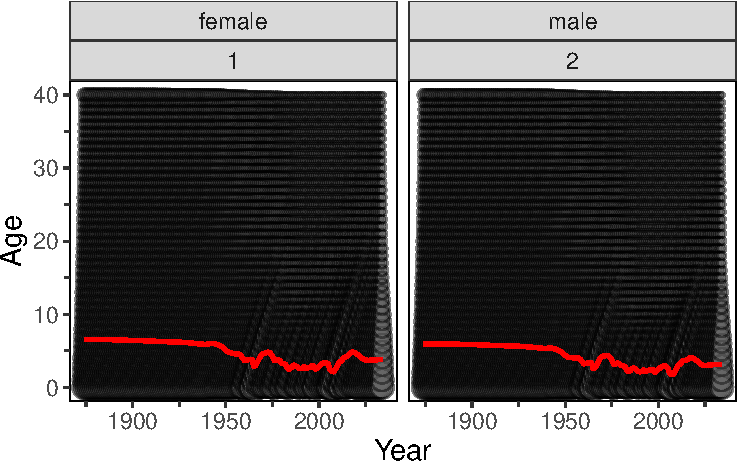
\includegraphics[keepaspectratio,alt={Bubble plot showing relative age proportions over time. The x axis shows the year, which spans from 1874 to 2034. The y axis shows age in years, which spans from 0 to 40. The size of the bubbles range from 0 to 19757.6.}]{sar_USWC_Petrale_sole_skeleton_files/figure-pdf/fig-abundance_at_age-1.pdf}}

}

\caption{\label{fig-abundance_at_age}Model estimate of population
numbers at age over time. The relative size of each bubble for a given
year and age indicates the relative abundance in that category compared
with others.}

\end{figure}%

\newpage{}

\begin{figure}

\centering{

\pandocbounded{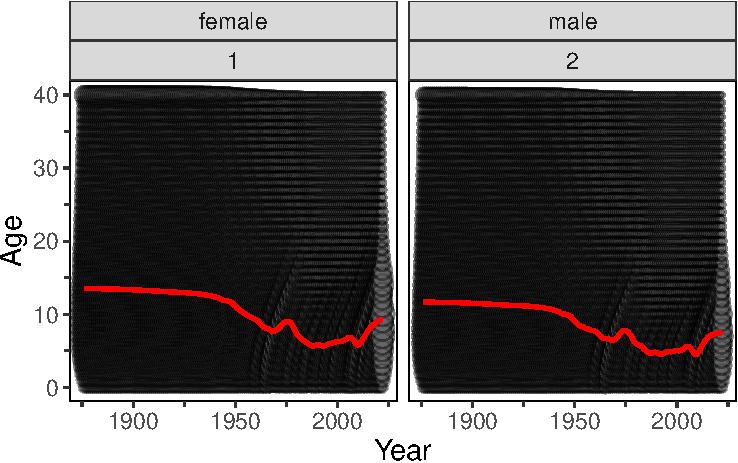
\includegraphics[keepaspectratio,alt={Bubble plot showing estimated population numbers at age and population biomass at age. The x axis shows the year, which spans from 1876 to 2022. The y axis shows age, which spans from 0 to 40. The size of the bubbles range from 0 to 3654.45.}]{sar_USWC_Petrale_sole_skeleton_files/figure-pdf/fig-biomass_at_age-1.pdf}}

}

\caption{\label{fig-biomass_at_age}Estimated population numbers at age
and population biomass at age over time. The relative size of each
bubble for a given year and age indicates the relative abundance or
biomass in that category compared with others.}

\end{figure}%

\newpage{}

\begin{figure}

\centering{

\pandocbounded{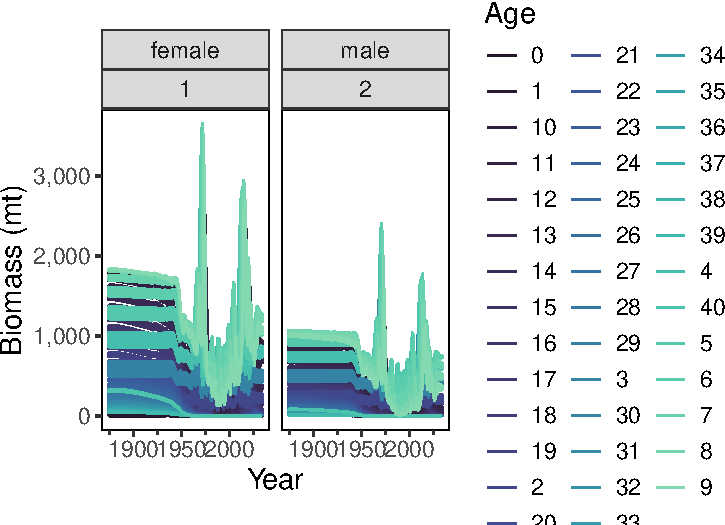
\includegraphics[keepaspectratio,alt={Line graph showing biomass time series. The x axis shows the year, which spans from 1874 to 2034. The y axis shows biomass in mt, which spans from 5.32659e-14 to 3654.45.}]{sar_USWC_Petrale_sole_skeleton_files/figure-pdf/fig-biomass-1.pdf}}

}

\caption{\label{fig-biomass}Biomass (B) time series. The horizontal
dashed line represents the limit reference point (msy mt).}

\end{figure}%

\newpage{}

\begin{figure}

\centering{

\pandocbounded{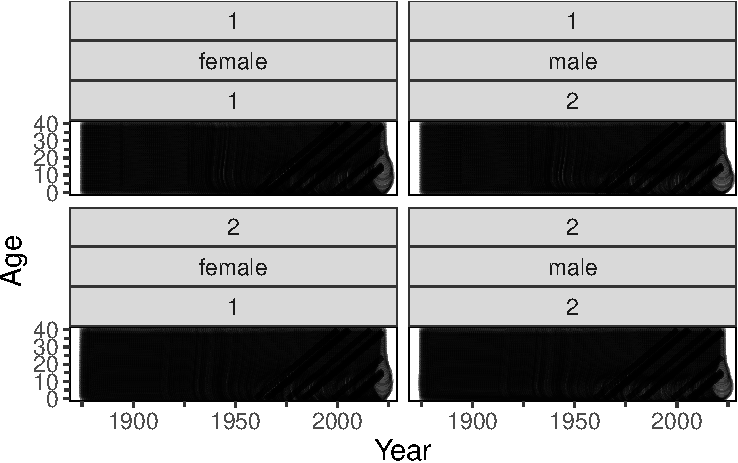
\includegraphics[keepaspectratio,alt={Bubble plot showing estimated total catch at age. The x axis shows the year, which spans from 1876 to 2022. The y axis shows age, which spans from 0 to 40. The size of the bubbles range from 0 to 540.076.}]{sar_USWC_Petrale_sole_skeleton_files/figure-pdf/fig-catch_comp-1.pdf}}

}

\caption{\label{fig-catch_comp}Fishery age composition (1876-2022). The
area of the circle is proportional to the catch. Diagonal lines
indicated the top 5\textbackslash\% strongest year classes.}

\end{figure}%

\newpage{}

\begin{figure}

\centering{

\pandocbounded{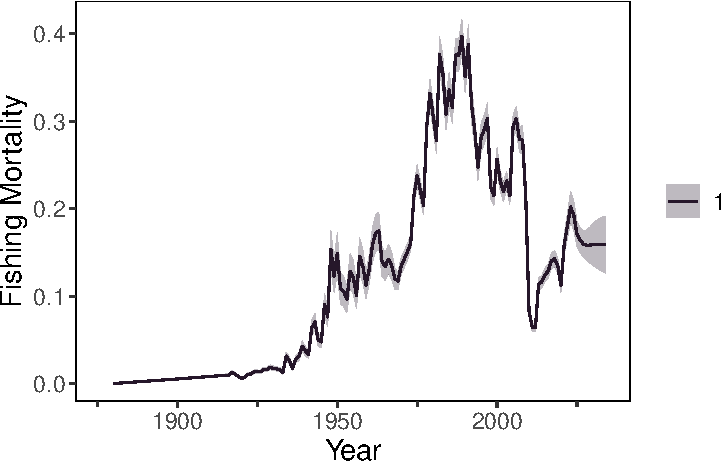
\includegraphics[keepaspectratio,alt={Line graph showing fishing mortality over time. The x axis shows the year, which spans from 1876 to 2034. The y axis shows fishing mortality, which spans from NA to NA.}]{sar_USWC_Petrale_sole_skeleton_files/figure-pdf/fig-fishing_mortality-1.pdf}}

}

\caption{\label{fig-fishing_mortality}Fishing mortality (F) over time.
The horizontal dashed line represents the target reference point (msy).}

\end{figure}%

\newpage{}

\begin{figure}

\centering{

\pandocbounded{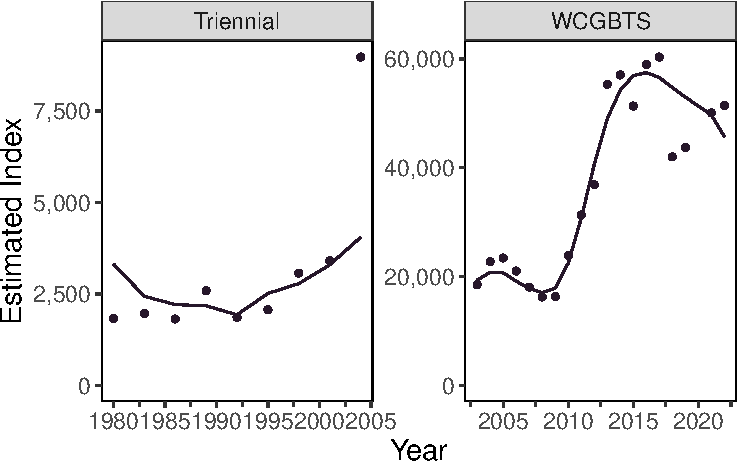
\includegraphics[keepaspectratio,alt={Line graph showing catch per unit effort (CPUE) over time, stratified by survey/fleet. The x axis shows the year, which spans from 1980 to 2022. The y axis shows CPUE in an estimated index ratio, which spans from 1819.1 to 60348.}]{sar_USWC_Petrale_sole_skeleton_files/figure-pdf/fig-index-1.pdf}}

}

\caption{\label{fig-index}Catch per unit effort (CPUE) over time for
fleet or survey. 95\textbackslash\% confidence intervals are shown for
each survey/fleet.}

\end{figure}%

\newpage{}

\begin{figure}

\centering{

\pandocbounded{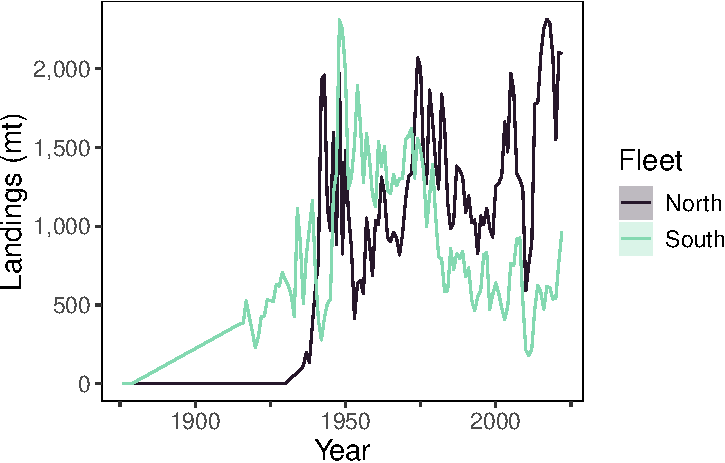
\includegraphics[keepaspectratio,alt={Cumulative area plot showing historical landings. The x axis shows the year, which spans from 1876 to 2022. The y axis shows landings in mt, which spans from 0 to 2313.91.}]{sar_USWC_Petrale_sole_skeleton_files/figure-pdf/fig-landings-1.pdf}}

}

\caption{\label{fig-landings}Historical landings by fleet.}

\end{figure}%

\newpage{}

\begin{figure}

\centering{

\pandocbounded{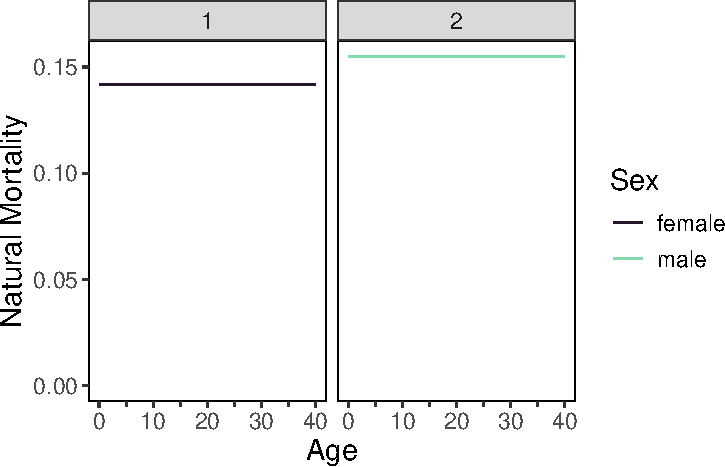
\includegraphics[keepaspectratio,alt={Line graph showing natural mortality. The x axis shows age in years, which spans from 0 to 40. The y axis shows the natural mortality rate per year, which spans from 0.142 to 0.155.}]{sar_USWC_Petrale_sole_skeleton_files/figure-pdf/fig-natural_mortality-1.pdf}}

}

\caption{\label{fig-natural_mortality}Natural mortality (M) for each
age.}

\end{figure}%

\newpage{}

\begin{figure}

\centering{

\pandocbounded{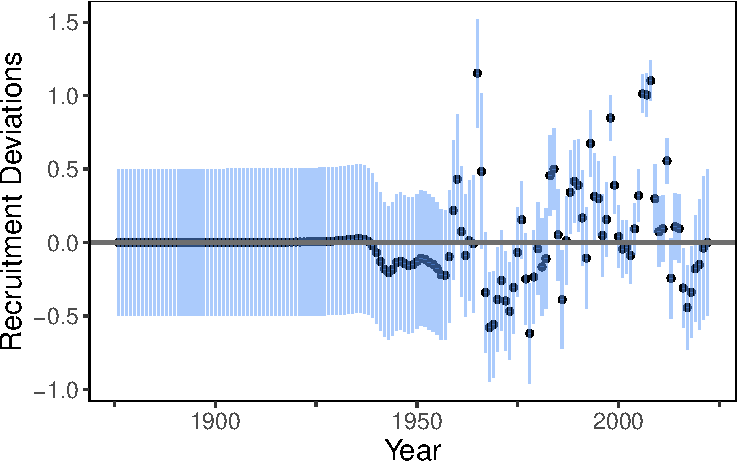
\includegraphics[keepaspectratio,alt={Scatterplot showing annual deviations in recruitment. Points have error bars and the dashed horizontal line at 0 represents no deviation from what would be estimated by the stock-recruit relationship. Positive values represent an increase in recruitment that year while negative values represent a decrease. The x axis shows year, which spans from 1876 to 2022. The y axis shows the recruitment deviation, which spans from -0.619 to 1.153 on a natural log scale.}]{sar_USWC_Petrale_sole_skeleton_files/figure-pdf/fig-recruitment_deviations-1.pdf}}

}

\caption{\label{fig-recruitment_deviations}Annual deviations (on natural
log scale) in the number of newly recruited fish the model estimates
each year.}

\end{figure}%

\newpage{}

\begin{figure}

\centering{

\pandocbounded{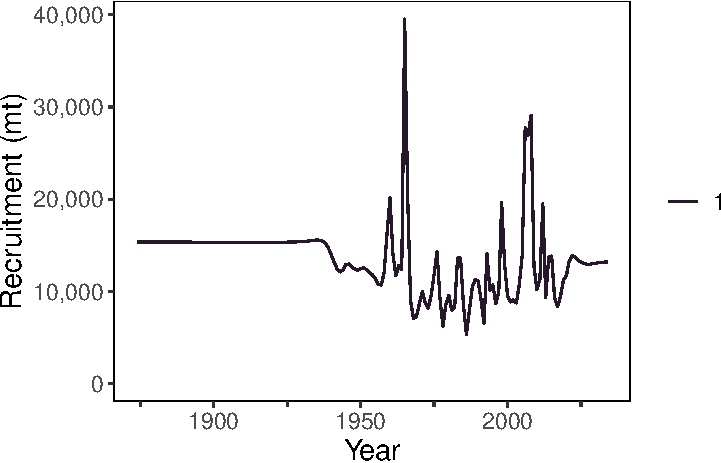
\includegraphics[keepaspectratio,alt={Line graph showing the assessment model estimated recruitment in mt for each year. The x axis shows years, which spans from 1874 to 2034. The y axis shows recruitment in mt, which spans from 5348.17 to 39515.1.}]{sar_USWC_Petrale_sole_skeleton_files/figure-pdf/fig-recruitment-1.pdf}}

}

\caption{\label{fig-recruitment}Estimated recruitment by the assessment
model each year in mt.}

\end{figure}%

\newpage{}

\begin{figure}

\centering{

\pandocbounded{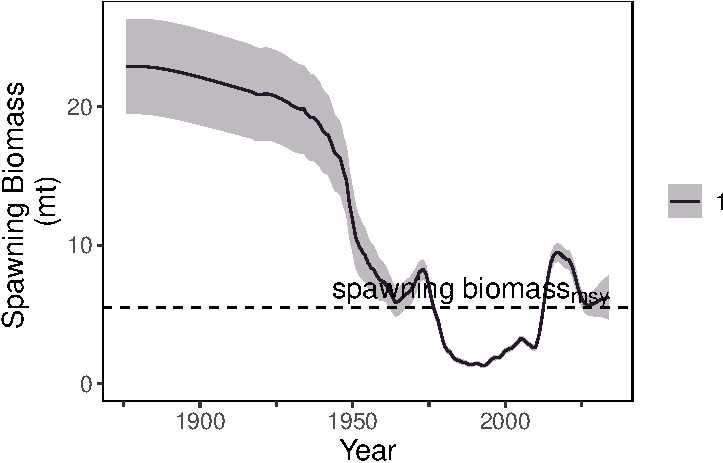
\includegraphics[keepaspectratio,alt={Line graph showing estimated spawning biomass. The x axis shows the year, which spans from 1876 to 2034. The y axis shows estimated spawning biomass in mt, which spans from 1.304 to 22.907.}]{sar_USWC_Petrale_sole_skeleton_files/figure-pdf/fig-spawning_biomass-1.pdf}}

}

\caption{\label{fig-spawning_biomass}Estimated spawning biomass (SB)
time series. The horizontal dashed line represents the spawning biomass
associated with the biomass limit reference point (msy mt).}

\end{figure}%

\newpage{}

\begin{figure}

\centering{

\pandocbounded{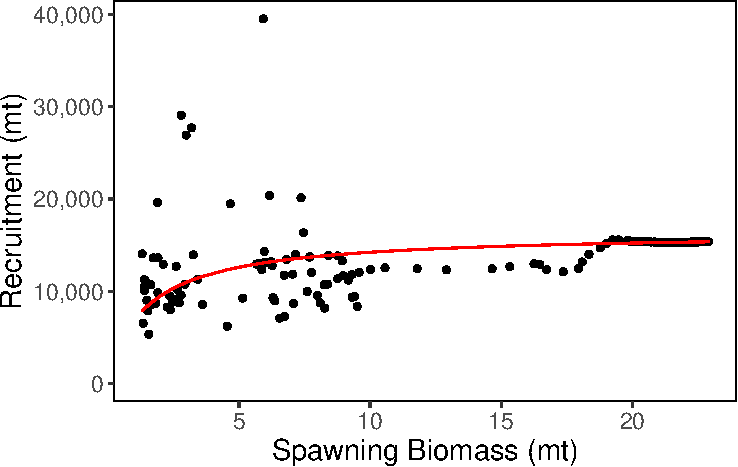
\includegraphics[keepaspectratio,alt={Point and line graph showing the relationship between stock biomass and newly recruited age 0 fish as estimated by the assessment model. Points represent model estimates of recruitment each year as a function of stock biomass, after adjusted by annual recruitment deviations. The line represents the best fit through the points for the stock relationship selected for use in the assessment model. The x axis shows spawning biomass in mt, which spans from 1.304 to 22.907. The y axis shows recruitment in mt, which spans from 5348.17 to 39515.1.}]{sar_USWC_Petrale_sole_skeleton_files/figure-pdf/fig-stock_recruitment-1.pdf}}

}

\caption{\label{fig-stock_recruitment}Stock recruitment relationship
estimated by the assessment model.}

\end{figure}%

\newpage{}




\end{document}
